\documentclass[12pt]{article}

% Packages
\usepackage{sbc-template}
\usepackage{graphicx,url}
\usepackage[brazil]{babel}   
\usepackage[utf8]{inputenc}  
\usepackage{lipsum}

\sloppy

% Info
\title{Albi:\\ A gro compiler to the SBML standard}
\author{Alek Frohlich\inst{1}, Gustavo Biage\inst{1}}
\address{Departamento de Informatica e Estatística – Universidade Federal de Santa Catarina \\
Florianopolis – SC – Brazil
  \email{\{alek.frohlich,gustavo.c.biage\}@grad.ufsc.br}
}

\begin{document}

\maketitle

\begin{abstract}
    The growth of research areas such as synthetic biology and systems biology leads to an increased willing to develop new, larger mathematical models to describe complex biological behavior. In order to enable natural flow of development of those models, scientists must have access to tools which increase the level of abstraction and enable reuse of biological components. Increased efforts are being put on solving these two problems. Thus, the present work tackles the question of reuse by integrating the existing programming language Gro with SBML for model interchangeability.
\end{abstract}

% Topics:
%       => What does albi fix that libSBML does not?
%       => What are the reasons we chose gro as albi's primary language?
%       => What are the disadvantages of the gro simulator
%       => What are the advantages of having the SBML model for a gro program?
\section{Introduction}

    Even though a Systems Biology Markup Language API library (LibSBML) has already been developed \cite{Bornstein2008}, it only ought to be useful in cases where a new model is to be developed. In cases where there is a preexisting model, on the other hand, the availability of a SBML library doesn't help much since the previous model would have to be entirely rewritten to fit the API. Instead, the present work proposes a language parser that generates SBML code from previously built gro models. gro is a language for programming, modeling, specifying and simulating the behavior of cells in growing micro colonies of microorganisms \cite{Jang2012}. It has been made the primary source of the parser considering it has many interesting syntactical constructs such as rate statements, program definitions and bacterial instantiation which can be neatly represented in SBML documents as reactions, local name spaces and compartments, respectively.
    
    % bad start
    % methods and attributes sounds bad
    Although gro's simulator has recently undergone a big improvement cycle, as seen in \cite{Gutirrez2017}, the language is still tightly coupled with it's simulator, making the models written in it chained to the methods and attributes of the simulator. Interfacing with SBML, on the other hand, possibilitates gro models to be run in any of the more than 100 simulators that support the Systems Biology Markup Language \cite{Hucka2007}.
    
    Another great opportunity the language was missing is BioModels integration \cite{LeNovere2006}. BioModels is a database of curated SBML and CellML models maintained with the intent of providing researches with models related to a particular disease, biological process or molecular complex. If gro code is to be translated into SBML, then models written in it are automatically more likely to be peer reviewed or stored as reference models for their respective biological behavior for which they describe.

\section{The parser}
    \lipsum[1]

\section{The Tellurium framework}
    \lipsum[1]

\section{Study case: The Repressilator}
    \lipsum[1]

\subsection{Mathematical Model}
    \lipsum[1]
    % Cite example
    \cite{Hucka2003}
    % Figure example
    (Figure~\ref{fig:repressilator}).

% Oscillation
\begin{figure}[ht]
\centering
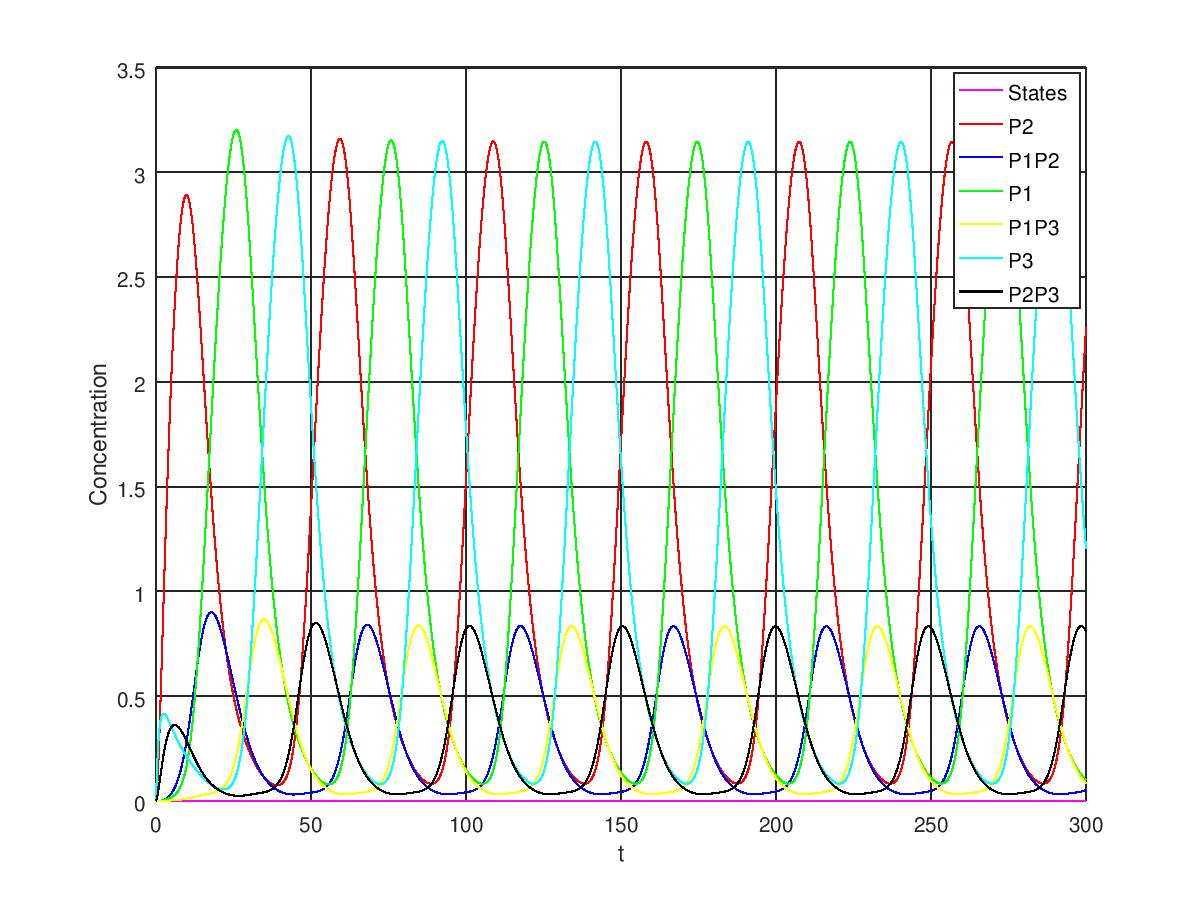
\includegraphics[width=.5\textwidth]{repressilator.jpg}
\caption{Repressilator}
\label{fig:repressilator}
\end{figure}

EPS generated from Octave
\begin{center}
    \begin{figure}[h]
        
        \begin{subfigure}
            \includegraphics[scale = 0.4]{my_plot-inc.eps}
            \caption{Caption1}
            \label{fig:subim1}
        \end{subfigure}
        \begin{subfigure}
            \includegraphics[scale = 0.4]{my_plot-inc.eps}
            \caption{Caption1}
            \label{fig:subim1}
        \end{subfigure}
    \end{figure}
    % \setlength{\unitlength}{1pt}
    % \begin{picture}(0,0)
    % \includegraphics[scale = 0.4]{my_plot-inc}
    % \end{picture}%
    % \begin{picture}(576,432)(0,0)
    % \fontsize{10}{0}
    % \end{picture}
\end{center}

\subsection{Extracting behavior from Gro}
    \lipsum[1]
    
\subsection{Simulating output on Copasi}
    \lipsum[1]

\section{Conclusion}
    \lipsum[1]
    
\section{Future works}
    \lipsum[1]

% References
\bibliographystyle{sbc}
\bibliography{sbc-template}

\end{document}
